% !TEX TS-program = pdflatex
% !TEX encoding = UTF-8 Unicode

% This is a simple template for a LaTeX document using the "article" class.
% See "book", "report", "letter" for other types of document.

\documentclass[10pt]{article} % use larger type; default would be 10pt
\usepackage[utf8]{inputenc} % set input encoding (not needed with XeLaTeX)
\usepackage{framed}
\usepackage[utf8]{inputenc}
\usepackage[T1]{fontenc}
\usepackage{csquotes}
\usepackage{booktabs}
\usepackage{wrapfig}
\usepackage[english]{babel}
\usepackage{blindtext}
\usepackage{subcaption}
\usepackage{lettrine}
%%% Examples of Article customizations
% These packages are optional, depending whether you want the features they provide.
% See the LaTeX Companion or other references for full information.

%%% PAGE DIMENSIONS
\usepackage{geometry} % to change the page dimensions
\setlength{\abovecaptionskip}{10pt plus 5pt minus 3pt}
\usepackage{wrapfig}
\geometry{a4paper} % or letterpaper (US) or a5paper or....
% \geometry{margin=2in} % for example, change the margins to 2 inches all round
% \geometry{landscape} % set up the page for landscape
%   read geometry.pdf for detailed page layout information

\usepackage{graphicx} % support the \includegraphics command and options
\usepackage{amsthm, amsmath, wasysym, MnSymbol}
\usepackage{booktabs} % Top and bottom rules for table
\usepackage[font=small,labelfont=bf]{caption} % Required for specifying captions to tables and figures
% \usepackage[parfill]{parskip} % Activate to begin paragraphs with an empty line rather than an indent

%%% PACKAGES

\usepackage{booktabs} % for much better looking tables
\usepackage{array} % for better arrays (eg matrices) in maths
\usepackage{paralist} % very flexible & customisable lists (eg. enumerate/itemize, etc.)
\usepackage{verbatim} % adds environment for commenting out blocks of text & for better verbatim
%\usepackage{subfig} % make it possible to include more than one captioned figure/table in a single float
% These packages are all incorporated in the memoir class to one degree or another...

%%% HEADERS & FOOTERS
\usepackage{fancyhdr} % This should be set AFTER setting up the page geometry
\pagestyle{fancy} % options: empty , plain , fancy
\renewcommand{\headrulewidth}{0pt} % customise the layout...
\lhead{}\chead{}\rhead{}
\lfoot{}\cfoot{\thepage}\rfoot{}
%%% SECTION TITLE APPEARANCE
\usepackage{sectsty}
\allsectionsfont{\sffamily\mdseries\upshape} % (See the fntguide.pdf for font help)
% (This matches ConTeXt defaults)

%%% ToC (table of contents) APPEARANCE
\usepackage[nottoc,notlof,notlot]{tocbibind} % Put the bibliography in the ToC
\usepackage[titles,subfigure]{tocloft} % Alter the style of the Table of Contents
\renewcommand{\cftsecfont}{\rmfamily\mdseries\upshape}
\renewcommand{\cftsecpagefont}{\rmfamily\mdseries\upshape} % No bold!

%%% END Article customizations

%%% The "real" document content comes below...
\font\loll= cmr25 at 45pt
\title{ \loll Thermal analysis on a turbulent Poiseuille flow}
\author{Felipe J. O. Ribeiro, Aristeu da Silveira Neto.}
%\date{} % Activate to display a given date or no date (if empty),
         % otherwise the current date is printed 

\begin{document}
\maketitle

%\begin{figure}[h!]
%	\centering
%	
\includegraphics[angle=0, trim={0 1cm 0 1cm},scale=0.70]{turbulence}
%	\label{turbulence}
%\end{figure}

\begin{abstract}
	\noindent Fluid dynamics is a subject of great academic and industrial interest. It offers many opportunities that require optimization in a variety of practical engineering problems. The modeling of thermal properties of turbulent flows is something of remarkable complexity, that can be explained mathematically by the chaotic nature of this non-linear differential analysis, fact beautifully stated in the Strogatz`s book "Nonlinear Dynamics and Chaos". The immediate result of such fact is the impossibility of an exact mathematical answer for, near, all real applications. The only way of gathering results, then, is by numerical approach, with the discretization of space and time, for an approximate result. The problem is that, in most cases, these are a so big computational problem that become inviable. With that in mind, the authors of the present paper aim to develop a semi-exact meta-modeled approach for a turbulent Poiseuille flow's thermal analysis over a channel, aiming on efficiency and accuracy when compared to the DNS solution, the most accurate but computationally expensive method. Such approach, presented in the present paper, resulted on a new adjusted model for the turbulent Prandtl and Cebeci numbers on Poiseuille channel flows.
\end{abstract} 

%\pagebreak
\vspace{8.0mm}

\begin{LARGE}
	Nomenclature: 
\end{LARGE} 


	Pr = Molecular Prandtl number
	
	$ Pr_t $ = Turbulent Prandtl number 
	
	A = Cebeci's constant
	
	
	$Re$ = Reynolds number, $Re = \frac{2R \overline{U}}{\nu}$
	
	
	$Re_\tau$ = Turbulent Reynolds number, $Re_\tau = \frac{R U_\tau}{\nu}$
	
	
	
	T = Temperature
	
	
	
	$T_\tau$ = Wall coordinate temperature, $T_\tau = \frac{q_w}{\rho c_p u_\tau}$ 
	
	
	
	
	$T_m$ = Bulk temperature 
	
	
	
	
	$T_w$ = Temperature on the walls
	
	
	
	
	$T^\ast$ = Difference of temperature, $T^\ast = T - t_w $ 
	
	
	
	
	${U}_c$ = Velocity on channels center
	
	
	
	u , v , w = Velocities components on each axis
	
	
	$u^\prime $ , $ v^\prime $ , $ w^\prime $ = Fluctuations of velocity on each axis
	
	
	$u_\tau$ = Friction velocity
	
	
	x , y , z = Cartesian classic coordinates
	
	
	$\tilde{y} $= Space nondimensionalization, $ y \frac{u_\tau}{R} $
	
	
	R = Half of the channel width
	
	
	
	b = Channel depth
	
	
	
	$\nu$ = Kinematic viscosity
	
	
	$\nu_\tau$ = Turbulent viscosity
	
	
	$\rho$ = Specific mass
	
	
	$\alpha$ = Thermal diffusivity
	
	
	$\alpha_t$ = Turbulent thermal diffusivity 
	
	\vspace{8.00mm}
	
	\begin{LARGE}
		Superscripts: 
	\end{LARGE} 
	
	$\tilde{()}$ = Normalized under wall properties
	
	$\overline{()}$ = Mean value
	 
	$()^\prime$ = Fluctuation value


\section{Introduction}

\lettrine[nindent=0em,lines=2]{I}t is well known that the field of turbulent regime is of such hight complexity that, even nowadays, it is not completely understood, as described by O. Basim and Hasan, 2007 \cite{hasan}. Out of the domain of Direct Numerical Simulations (DNS), all sorts of numerical approximations have to be assumed to properly mathematically develop the Navier-Stokes equations. The nonlinear behavior of these systems \cite{John} make difficult for an exact mathematical solution. 

Despite the difficulty, a big part of the scientific community is studying turbulence on fluid and thermal dynamics, because of the great industrial and academic interest, as the problem offers great opportunities in optimization of machinery. In other hand, it is an example of chaotic nonlinear dynamic system, what grows in the eyes of academia.   

In the present work, the mixing length model, by Ludwig Prandtl, was used, and it relies on the Boussinesq hypothesis for being a way of modeling the Reynolds shear tensor and to close the filtered Navier-Stokes and energy equations.

In this context, some parameters that worth mentioning are the turbulent Prandtl number \cite{Prandtl} and the constant $A = 26$, on Cebeci`s damping formulation \cite{Cebeci}. These parameters are used for modeling important properties of the fluid`s thermal diffusion and dynamics as said by Silveira-Neto, 2018 \cite{aristeu}. Such parameters are examples of approximations that are necessary to implement a modeling method, like RANS, URANS and LES \cite{aristeu}. It consists in not numerically resolving the Naiver-Stokes equation on all scales required, but instead substituting some tensors and other nonlinear therms by conceptual and experimental approximations.

Such methods are important because they offer a much quicker solution. The DNS approach demands high computational work, not even being possible or viable in some cases, as explained on H. Kawamura, H. Abe and Yuichi Matsuo's work \cite{Abe}. An example of this is for high Reynolds number flows. But, in other hand, these approximated methods result in some errors in comparison with the DNS solution.    

On the present paper, the authors aim to develop a semi analytical RANS (Reynold`s Averaged Navier-Stokes) method, with the averaged energy equation, to describe the thermal configuration on turbulent plane Poiseuille flows \cite{Poiseuille}, modeled with the mixture length methodology. Meta-models were developed defining the turbulent Prandtl number \cite{Prandtl} and the constant $A = 26$, on Cebeci`s damping formulation, to enhance the results compared to DNS solutions, resulting on accuracy and efficiency, what gave birth to new models for the parameters modeled. The results of this work's formulation were compared with the DNS result (\cite{DNS1020} , \cite{DNS150}), aiming to provide an analysis on the viability of meta models on Poiseuille turbulent flows with thermal effects. \\       
 

\section{Physical model}

The problem was defined as a plane channel flow, with only one finite dimension on the $y$ axis. Two boundary walls were set as nonslip infinite plates and in a constant thermal flux regime. The $z$ axis was proposed self similar both on velocity and temperature, resulting on a plane domain (Fig.\ref{figure.1}). \\
The flow was considered incompressible and the fluid was considered Newtonian. The fluid flows, in average, on the $x$ axis direction. \\
The Reynolds numbers ranges from $4560$ to $41441$, resulting on a turbulent regime. 

\begin{figure}[h!]
	\centering
	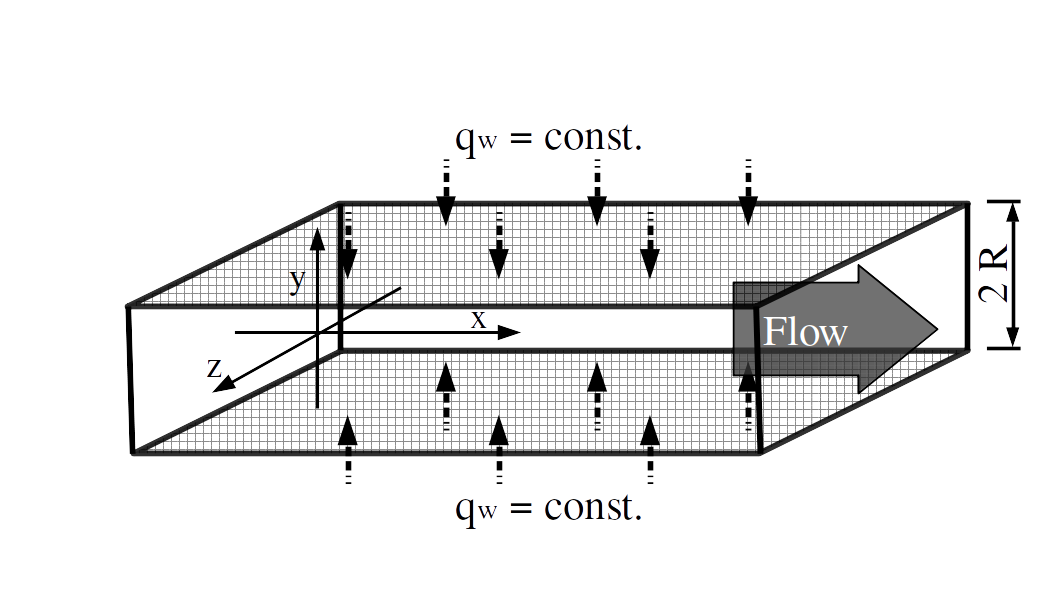
\includegraphics[angle=0, trim={0mm 10mm 0mm 20mm}, clip , scale=0.40]{fotos_formatacao_final/canal1}
	\caption{Geometric definition and boundary condition of the system.}
	\label{figure.1}
\end{figure}

The base mathematical formulation for the problem where the continuity, Navier-Stokes equations, as presented on Cengel's book \cite{Cengel}, and the thermal energy transport equation, as presented on Freank's Incropera \cite{Incropera}. These were the assumptions made to the proposed problem, that will be considered on the differential mathematical model ahead.









\section{Differential mathematical model}

The mean continuity (Eq.\ref{mass}), the mean Navier-Stokes (Eq.\ref{dynamics}) and the mean thermal energy (Eq.\ref{energy permanent}) equations are presented as follows: 


\begin{equation}\label{mass}
\frac{\partial \overline{u}}{\partial x} = 0,
\end{equation}

\begin{equation}\label{dynamics}
\frac{\partial \overline{u} \, \overline{v}}{\partial y} = 
- \frac{1}{\rho} \frac{\partial \overline{p}}{\partial x} + \frac{\partial}{\partial y}\left(\nu \frac{\partial \overline{u}}{\partial y} - \overline{u^\prime v^\prime}\right),
\end{equation}


\begin{equation}\label{energy permanent}
\frac{\partial{}}{\partial{x}} \left(\overline{T^\prime u^\prime}\right) + \frac{\partial{}}{\partial{x}}\left(\overline{u} \overline{T}\right)     + 
\frac{\partial{}}{\partial{y}} \left(\overline{T^\prime v^\prime}\right) + \frac{\partial{}}{\partial{y}}\left(\overline{v} \overline{T}\right) 
=
{\frac{\partial{}}{\partial{x}}} \left(\alpha {\frac{\partial{\overline{T}}}{\partial{x}}} \right) +
{\frac{\partial{}}{\partial{y}}} \left(\alpha {\frac{\partial{\overline{T}}}{\partial{y}}} \right). 
\end{equation}


The time independence and mean characterization of the system configure the method known as Reynolds Averaged Navier Stokes (RANS) methodology.

\subsection{The temperature permanent regime}

The velocity field is completely developed on the channel, for mean values (Fig.\ref{figure.3}), but this is not the case for the temperature field, as a constant thermal flux is imposed over the walls.\\
Even considering the mean values, the temperature field of a turbulent channel flow don't converge naturally to a unidimensional permanent state (Fig.\ref{figure.2}).

In a effort to simplify the solution, the thermal configuration was studied with a thermal energy balance (Eq.\ref{c_h_e}).
\begin{figure}[h!]
	\centering
	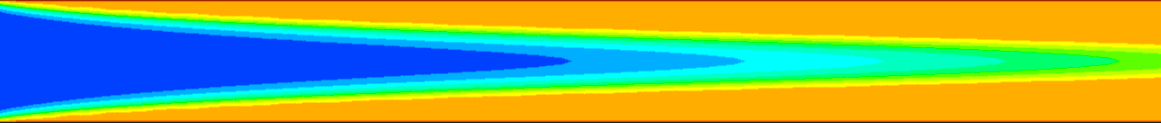
\includegraphics[angle=0, scale=0.40]{fotos_formatacao_final/temperatura}
	\caption{Temperature field in statistical permanent regime inside a plane channel.}
	\label{figure.2}
\end{figure}
\begin{figure}[h!]
	\centering
	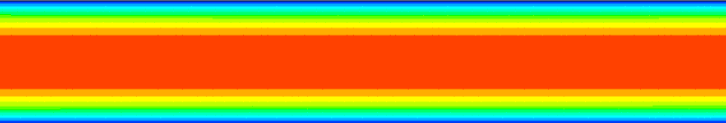
\includegraphics[angle=0, height=1.4cm , width=12.3cm]{fotos_formatacao_final/velocidade}
	\caption{Velocity field in statistical developed regime inside a plane channel.}
	\label{figure.3}
\end{figure}


\begin{equation}\label{c_h_e}
q_{conv.} = \dot{m} C_p \Delta T_m,
\end{equation}
\begin{equation}
2q_w b \Delta x = \dot{m} C_p \Delta T_m,
\end{equation}\\


{\parindent0pt where $b$ is the depth of the channel and $T_m$ the average temperature in a cross-section. So, substituting $ \dot{m} = u_m 2R b \rho $, and assuming $ \Delta T_m = \frac{\partial{\left(\overline{T}_m\right)}}{\partial{x}} \Delta x $:}

\begin{equation}
2q_w b \Delta x = u_m 2R b \rho  C_p \frac{\partial{\left(\overline{T}_m\right)}}{\partial{x}} \Delta x,
\end{equation}     
\begin{equation}
q_w = u_m R \rho  C_p \frac{\partial{\left(\overline{T}_m\right)}}{\partial{x}} ,
\end{equation} 
\begin{equation}\label{c_h_ee}
\frac{\partial{\left(\overline{T}_m\right)}}{\partial{x}} = \frac{q_w}{u_m  R \rho  C_p } .
\end{equation} 

As all therms on the right side are constants, the mean temperature had to varies linearly on the stream-wise direction.  
To better understand the wall temperature with such energy profile, a convective thermal formulation was used, which can be expressed mathematically by:
\begin{equation}
q_w = h A \left( T_w(x) - \overline{T}_m(x)\right).
\end{equation}
It should be observed that $h$ is constant since this is a fully dynamically developed flow. Thus, using Eq.(\ref{c_h_ee}), it is possible to write:
%\begin{equation}
%T_w(x) - \overline{T}_m(x) = \frac{q_w}{hA}.
%\end{equation}
%\begin{equation}
%\frac{d T_w(x)}{d x} - \frac{d \overline{T}_m(x)}{d x} = \frac{d \frac{q_w}{hA}}{dx}.
%\end{equation}
\begin{equation}
\frac{d T_w(x)}{d x} = \frac{d \overline{T}_m(x)}{d x} = Cte.
\end{equation}	

With the temperature on the walls and the mean temperature gradient set as linear by these mathematical statements, it was possible to extend this gradient to all the domain considering the boundary conditions and the symmetry of the system. So a constant temperature gradient was imposed on the heated walls creating a boundary condition of constant thermal flux, resulting on all the temperature field to varies linearly on the $x$ axis. The temperature value was then decomposed to the form $ T^\ast(y) = T(x,y) - T_w(x) $ where $T_w(x)$ is the temperature at the wall, resulting in a similarity effect on the streamwise direction, resuming the problem to a unidimensional representative state for the variable $T^\ast(y)$. Therefore, this decomposition was replaced in (\ref{energy permanent}):



\begin{equation}
\begin{split}
\frac{\partial{}}{\partial{x}} \left(\overline{(T^\ast + T_w)^\prime} \overline{ u^\prime}\right) + \frac{\partial{}}{\partial{x}}\left(\overline{(T^\ast + T_w)} \overline{u}\right)+ 
\frac{\partial{}}{\partial{y}} \left(\overline{(T^\ast + T_w)^\prime} \overline{ v^\prime}\right) + \frac{\partial{}}{\partial{y}}\left(\overline{(T^\ast + T_w)} \overline{v}\right) = \\
{\frac{\partial{}}{\partial{x}}} \left(\alpha {\frac{\partial{\overline{(T^\ast + T_w)}}}{\partial{x}}} \right) +
{\frac{\partial{}}{\partial{y}}} \left(\alpha {\frac{\partial{\overline{(T^\ast + T_w)}}}{\partial{y}}} \right). 
\end{split}
\end{equation}

Then the expression could be further developed algebraically considering all mean velocity on $y$ and $z$ axis null:

\begin{equation}\label{equation_var}
{\frac{\partial{}}{\partial{y}}} \left(\alpha {\frac{\partial{\overline{T^\ast}}}{\partial{y}}}   
- \left(\overline{ T^{\ast\prime} v^\prime}\right) \right)
= 
\overline{u}\frac{\partial{}}{\partial{x}}\left(\overline{T_w}\right).
\end{equation}



\subsection{The Boussinesq hypothesis}

Now, on a unidimensional simplified expression, the model requires a closure model for the turbulent flux of thermal energy. \\
So the Boussinesq hypothesis was used. The term $\overline{T^{\ast\prime}  v^\prime}$ can be modeled with:
\begin{equation}\label{bou}
-\left(\overline{ T^{\ast\prime}  v^\prime}\right) = 
\alpha_t \frac{\partial{\overline{T^\ast}}}{\partial{y}}.
\end{equation}
Thus, the following equation can be obtained by substituting in the main equation (\ref{equation_var}):
\\
\begin{equation}
{\frac{\partial{}}{\partial{y}}} \left[(\alpha + \alpha_t)  \frac{\partial \overline{T^\ast}}{\partial y} \right]
= 
\overline{u}\frac{\partial{}}{\partial{x}}\left(\overline{T_w}\right) . 
\end{equation}

\subsection{Prandtl mixing length model} 

The term of the turbulent thermal diffusion, $\alpha_t$, needs to be modeled. \\
The classical concept of the turbulent Prandtl number is used in the present work:
\begin{equation}
Pr_t = \frac{\nu_t}{\alpha_t}.
\end{equation} 
The term $ \nu_t $ need to be modeled. The value of the turbulent Prandtl number $ Pr_t = 0.71 $ has been used in the literature.
With the model of the Prandtl mixing length, it is postulated that:
\begin{equation}
\nu_t = {l^2_m} \left| \frac{\partial \overline{u}}{\partial y} \right|.
\end{equation}
The mixing length introduces a module into the differential model as well as the parameter turbulent Prandtl number:
\\
\begin{equation}
{\frac{\partial{}}{\partial{y}}} \left( \left( \alpha   
+ \frac{\nu_t}{Pr_t} \right) \frac{\partial \overline{T^\ast}}{\partial y} \right)
= 
\overline{u}\frac{\partial{}}{\partial{x}}\left(\overline{T_w}\right)  .
\end{equation}
\begin{equation}\label{equationquasela}
{\frac{\partial{}}{\partial{y}}} \left( \left( \alpha   
+ \frac{{l^2_m} \left| \frac{\partial \overline{u}}{\partial y} \right|}{Pr_t} \right) \frac{\partial \overline{T^\ast}}{\partial y} \right)
= 
\overline{u}\frac{\partial{}}{\partial{x}}\left(\overline{T_w}\right)  .
\end{equation}
\\

It is possible to notice, when analyzing the dynamics of the flow, that for positive values of $ y $, see figure \ref{figure.1}, the first derivative of velocity will always be negative, since we have a velocity that decreases with the increase of $ y $. It result:\\
\begin{equation}
{\frac{\partial{}}{\partial{y}}} \left( \left( \alpha   
- \frac{{l^2_m}}{Pr_t}\frac{\partial \overline{u}}{\partial y} \right) \frac{\partial \overline{T^\ast}}{\partial y} \right)
= 
\overline{u}\frac{\partial{}}{\partial{x}}\left(\overline{T_w}\right)  .
\end{equation}



\subsection{The mixing length}

The mixing length $ l_m $ needs to be modeled. It can be observed that the experimental studies of Nikuradse was used in order to model this parameter for channel flows, as follows:
\begin{equation}
L\left(\frac{y}{R}\right) = \frac{l_m}{R} = 0.14 - 0.08 \left(\frac{y}{R}\right)^2 - 0.06\left(\frac{y}{R}\right)^4.
\end{equation}
To further completeness of the model, Cebeci and Bradshaw added the Van Driest damping function:
\begin{equation}\label{eqution_mixturelength}
L\left(\frac{y}{R}\right)  = \frac{l_m}{R} = \left\{ 0.14 - 0.08 \left(\frac{y}{R}\right)^2 - 0.06\left(\frac{y}{R}\right)^4\right\}\left\{  1 - e^{[(\tilde{y} - 1) \frac{Re_\tau}{A}]}\right\},
\end{equation}
with $A = 26$ as the Cebeci`s constant. Thus, we had the mixing length defined by:
\begin{equation}
l_m = L R,
\end{equation}
$ L $ being a function in the $ y $ axis, given by equation (\ref{eqution_mixturelength}). So equation (\ref{equationquasela}) can be rewritten as:
\begin{equation}\label{cebeciconstant}
{\frac{\partial{}}{\partial{y}}} \left( \left( \alpha   
- \frac{{L}^2 R ^2}{Pr_t}\frac{\partial \overline{u}}{\partial y} \right) \frac{\partial \overline{T^\ast}}{\partial y} \right)
= 
\overline{u}\frac{\partial{}\left(\overline{T_w}\right)  }{\partial{x}}.
\end{equation}
 To compare the present work with literature models, this equation was nondimensionalized using the wall coordinates. It was considered: $ \tilde{y} = \frac{y . Re_\tau}{R} $, $ \tilde{\overline{u}} = \frac{\overline{u}}{u_\tau} $ , $ \tilde{\overline{T}} = \frac{\overline{T}}{T_\tau} $ , $ \tilde{\overline{T^\ast}} = \frac{\overline{T^\ast}}{T_\tau} $ , $Re_\tau = \frac{u_\tau R}{\nu}$, $Pr_t = \frac{\nu_t}{\alpha_t}$, $Pr = \frac{\nu}{\alpha}$, $T_\tau = \frac{q_w}{\rho C_p u_\tau}$, $\frac{\partial{\left(T_m\right)}}{\partial{x}} = \frac{q_w}{u_m  R \rho  C_p } $ and $\frac{\partial \overline{p}}{\partial x} = - \frac{u_\tau^2 \rho}{R} $. It results:
\\
\begin{equation}\label{equationultima}
{\frac{\partial{}}{\partial{\tilde{y}}}} \left( \left( \frac{Re_\tau}{Pr}   
- \frac{{L}^2 Re_\tau ^3}{Pr_t}\frac{\partial \tilde{\overline{u}}}{\partial \tilde{y}} \right) \frac{\partial \tilde{\overline{T^\ast}}}{\partial \tilde{y}} \right)
= 
\frac{\tilde{\overline{u}}}{\tilde{u_m}}.
\end{equation}
It is important to note that there is the velocity in the equation (\ref{equationultima}), that is, for the development of the thermal problem, the development of the dynamic channel profile is necessary. For this, a previously established RANS methodology \cite{Luigi} was used, as follows:
\begin{equation}\label{finalequationvelocity}	
\frac{\partial \tilde{\overline{u}}}{\partial \tilde{y}} = - \frac{2 \tilde{y} \frac{1}{Re_\tau} }{ 1 + \sqrt{ 1 + 4 L ^2 Re_\tau ^2 \tilde{y}}}.
\end{equation}	
This way, we had the first derivative of velocity in an continuous form.


\section{Numerical and algebraic models proposition}


To discretize the differential equation, an Eulerian domain was formulated. For the velocity a fourth-order Runge-kutta method was applied, while the temperature was arranged in a central differences scheme that had to be solved implicitly. The dynamic model is solved first, and its numerical result are used in the solution of the thermal profile. The cell center was used in a such way that the wall was placed at the cell center, and a point between cells was placed in the center of the channel. The convergence of the numerical results is shown in figure \ref{sistema}.
\begin{figure}[!h]
	\centering
	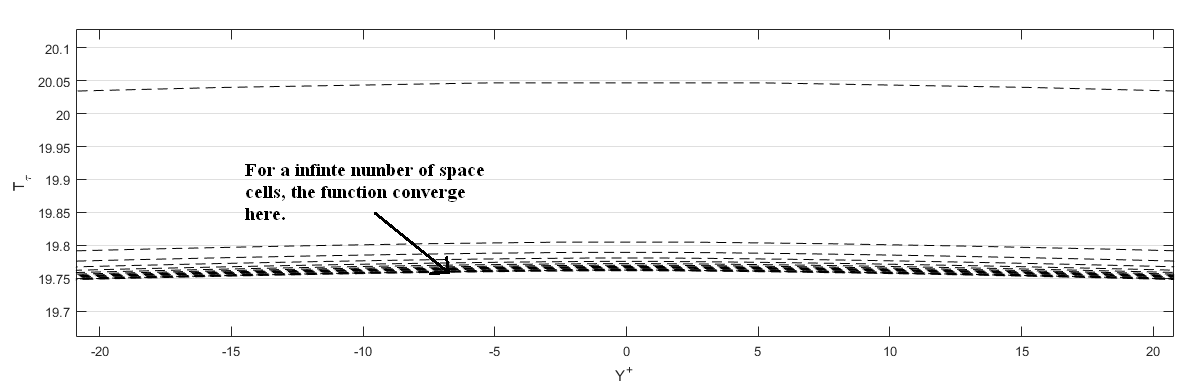
\includegraphics[angle=0, trim={5mm 0mm 0mm 0mm}, clip , scale=0.5]{convergnciaprimeira}
	\caption{The convergence of the numerical methodology up to 400 cells, with $Re_\tau = 1020$.}
	\label{sistema}
\end{figure}

\subsection{Preliminary results}
Initially the turbulent Prandtl number, $Pr_t = 0.71$, was used as in the literature. The obtained results presented in figure \ref{figuraresultados1} are compared with DNS from \cite{DNS1020} and \cite{DNS150}, using the norm L2.\\
	\begin{figure*}[h!] 
		\centering
%		\begin{subfigure}[t]{0.49\textwidth}
%		\centering
%		\includegraphics[angle=0, scale=0.32]{fotos_formatacao_final/Temperature_150_0025_classico}
%		\caption{Temperature configuration for $Re_\tau = 150$, $Pr = 0.025$, $L2 = 0.13$ }
%		\end{subfigure}%
		\begin{subfigure}[t]{0.49\textwidth}
		\centering
		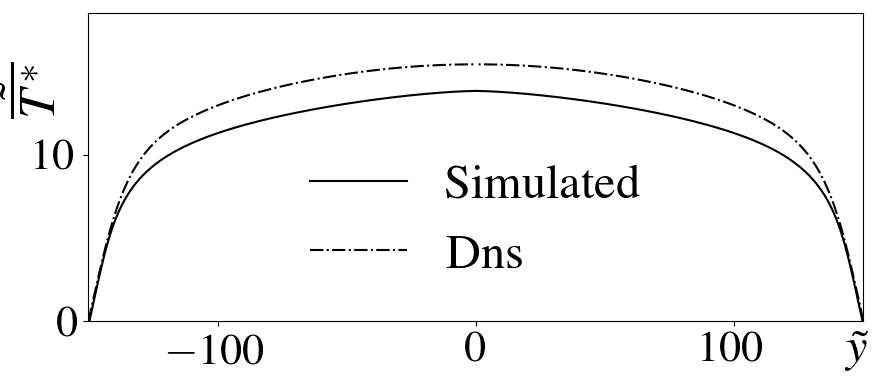
\includegraphics[angle=0, scale=0.24]{fotos_formatacao_final/Temperature_150_071_classico}
		\caption{$Re_\tau = 150$, $L2_t = 1.42$}
		\end{subfigure}
%		\begin{subfigure}[t]{0.49\textwidth}
%		\centering
%		\includegraphics[angle=0, scale=0.32]{fotos_formatacao_final/Temperature_395_0025_classico}
%		\caption{Temperature configuration for $Re_\tau = 395$, $Pr = 0.025$, $L2 = 0.52$}
%		\end{subfigure}%
		\begin{subfigure}[t]{0.49\textwidth}
		\centering
		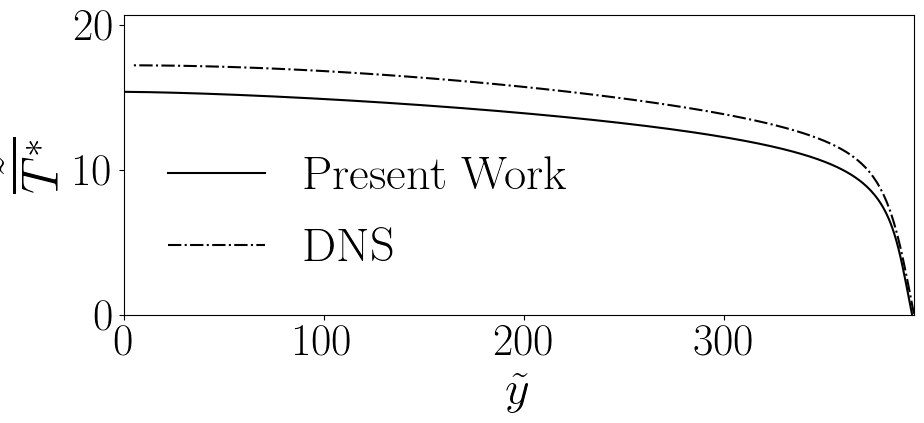
\includegraphics[angle=0, scale=0.24]{fotos_formatacao_final/Temperature_395_071_classico}
		\caption{$Re_\tau = 395$, $L2_t = 1.55$}
		\end{subfigure}
%		\centering
%		\begin{subfigure}[t]{0.49\textwidth}
%		\centering
%		\includegraphics[angle=0, scale=0.32]{fotos_formatacao_final/Temperature_395_1_classico}
%		\caption{Temperature configuration for $Re_\tau = 395$, $Pr = 1.0$, $L2 = 1.89$}
%		\end{subfigure}%
%		\begin{subfigure}[t]{0.49\textwidth}
%		\centering
%		\includegraphics[angle=0, scale=0.32]{fotos_formatacao_final/Temperature_395_2_classico}
%		\caption{Temperature configuration for $Re_\tau = 395$, $Pr = 2.0$, $L2 = 2.60$}
%		\end{subfigure}\\
%		\begin{subfigure}[t]{0.49\textwidth}
%		\centering
%		\includegraphics[angle=0, scale=0.32]{fotos_formatacao_final/Temperature_395_5_classico}
%		\caption{Temperature configuration for $Re_\tau = 395$, $Pr = 5.0$, $L2 = 3.75$}
%		\end{subfigure}%
%		\begin{subfigure}[t]{0.49\textwidth}
%		\centering
%		\includegraphics[angle=0, scale=0.32]{fotos_formatacao_final/Temperature_395_7_classico}
%		\caption{Temperature configuration for $Re_\tau = 395$, $Pr = 7.0$, $L2 = 4.24$}
%		\end{subfigure}\\
%	    \centering
%		\begin{subfigure}[t]{0.49\textwidth}
%		\centering
%		\includegraphics[angle=0, scale=0.32]{fotos_formatacao_final/Temperature_395_10_classico}
%		\caption{Temperature configuration for $Re_\tau = 395$, $Pr = 10.0$, $L2 = 4.55$}
%		\end{subfigure}%
%		\begin{subfigure}[t]{0.49\textwidth}
%		\centering
%		\includegraphics[angle=0, scale=0.32]{fotos_formatacao_final/Temperature_640_0025_classico}
%		\caption{Temperature configuration for $Re_\tau = 640$, $Pr = 0.025$, $L2 = 0.84$}
%		\end{subfigure}\\
		\begin{subfigure}[t]{0.49\textwidth}
		\centering
		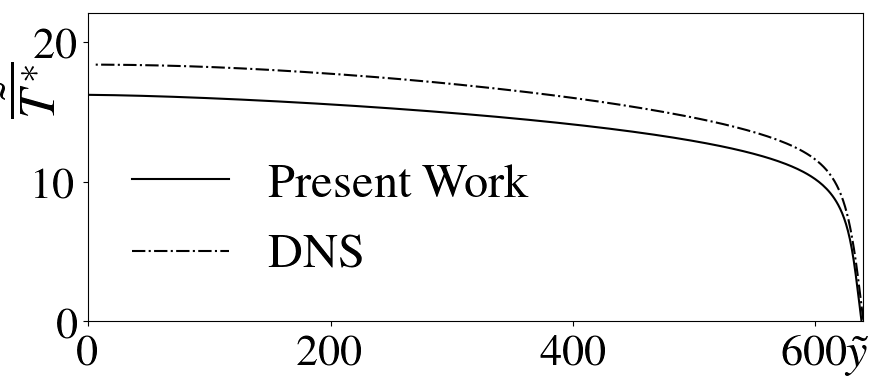
\includegraphics[angle=0, scale=0.24]{fotos_formatacao_final/Temperature_640_071_classico}
		\caption{$Re_\tau = 640$, $L2_t = 1.79$}
		\end{subfigure}%
		\begin{subfigure}[t]{0.49\textwidth}
		\centering
 		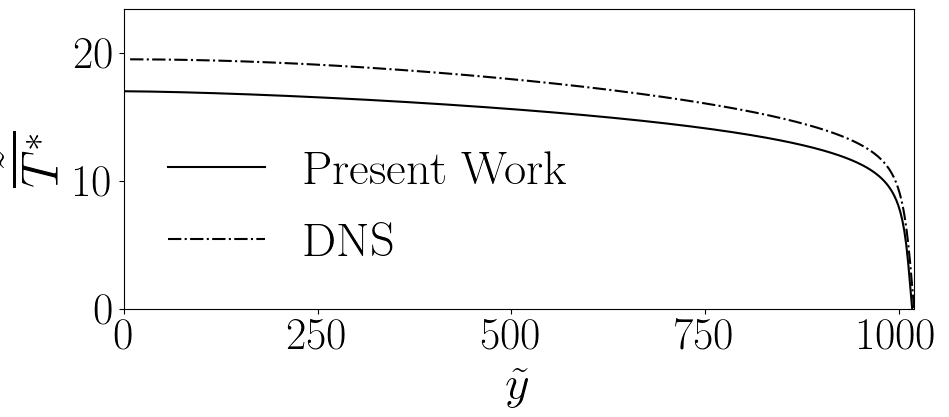
\includegraphics[angle=0, scale=0.24]{fotos_formatacao_final/Temperature_1000_071_classico}
		\caption{$Re_\tau = 1020$, $L2_t = 2.04$}
		\end{subfigure}%
		\caption{Temperature distribution for $Pr_t = 0.71$, $A = 26$ and $Pr = 0.71$} 
		\label{figuraresultados1}
	\end{figure*}	

First results weren't satisfactory. It was noticed that the turbulent Prandtl number had great influence on the outcome, so the turbulent Prandtl number from the DNS (figure \ref{figure5}) was used as a parameter in the program, obtaining an L2 norm of $ 0.19 $ to $ Re_t = 640 $. Thus it was identified that the problem was in the parametrization of the turbulent Prandtl number. It became the focus of the present research.

\begin{figure*}[h!]
	\centering
	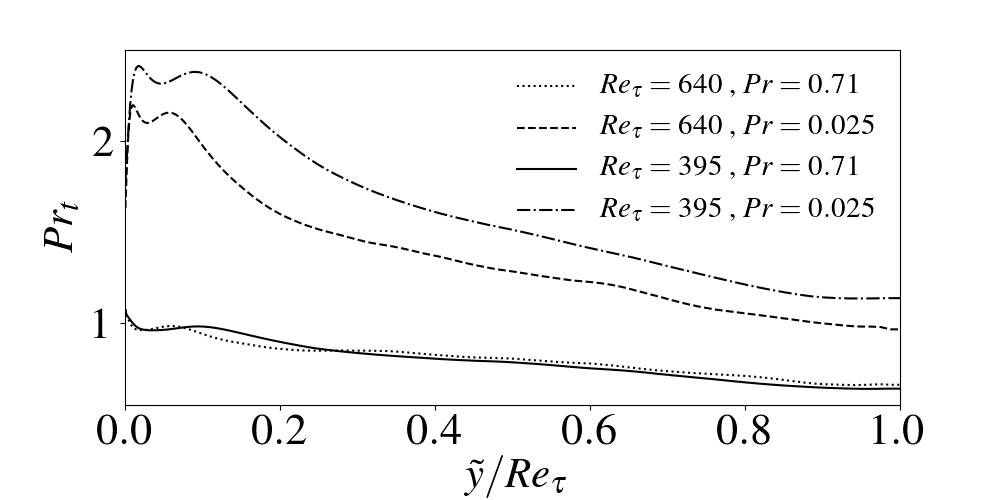
\includegraphics[angle=0, scale=0.45]{fotos_formatacao_final/DNS_PRt}
	\caption{Turbulent prandtl number from DNS in function of $ \tilde{y}/Re_\tau $ in the channel.}
	\label{figure5}
\end{figure*}

Thus, the effort to propose a parameterization adjusted for the turbulent Prandtl number started.
In this sense it was tried to adjust a value for which the error was minimal, comparing to the DNS. In this regards, the differential evolution algorithm methodology was applied. 



\subsection{The meta-modeling, with the genetic algorithm: Differential Evolution (DE)}
It was used an algorithm that searched for a minimal error for the given function, considering the turbulent Prandtl number as an editable variable and the smaller error as the pattern of interest.
It was obtained a turbulent Prandtl number of $ 0.9$ , for the Reynolds number $ Re_\tau = 1020$.
\begin{figure}[!h]
	\centering
	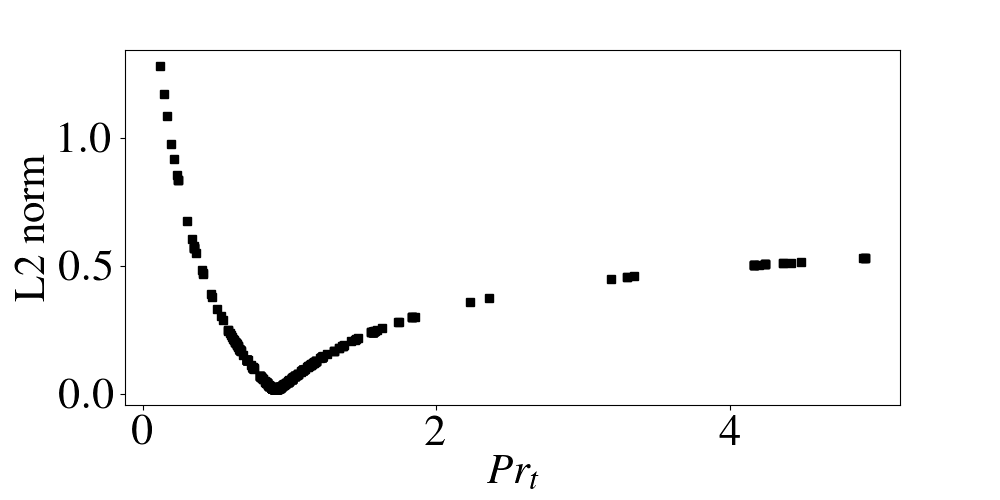
\includegraphics[angle=0, scale=0.35]{fotos_formatacao_final/Genetic_amostra}
	\caption{Genetic algorithm iterations, with simulations for $Re_\tau = 1020$. Convergence on $Pr_t = 0.9 $.}
\end{figure}

The turbulent Prandtl number obtained, $Pr_t = 0.9$, was considered to the others turbulent Reynolds numbers, resulting on figure \ref{primeiros}.
\begin{figure*}[!h]
	\centering
	\begin{subfigure}[t]{0.5\textwidth}
		\centering
		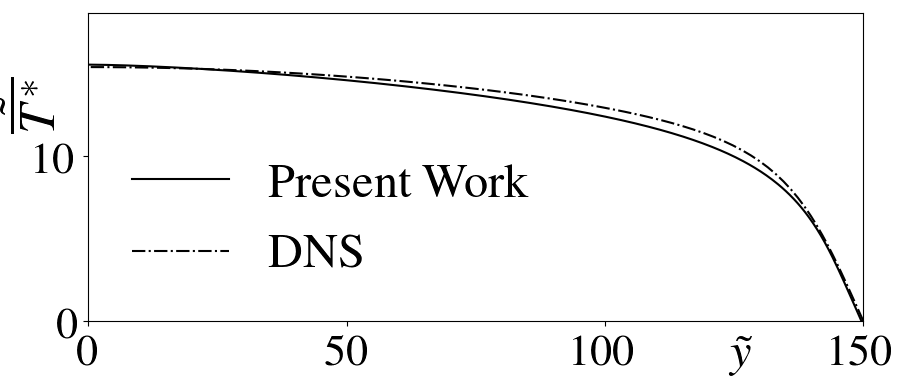
\includegraphics[angle=0, scale=0.24]{fotos_formatacao_final/Temperature_150_071_Prt0905_A26}
		\caption{$Re_\tau = 150$, $L2_t = 0.34$}
	\end{subfigure}
	\begin{subfigure}[t]{0.45\textwidth}
		\centering
		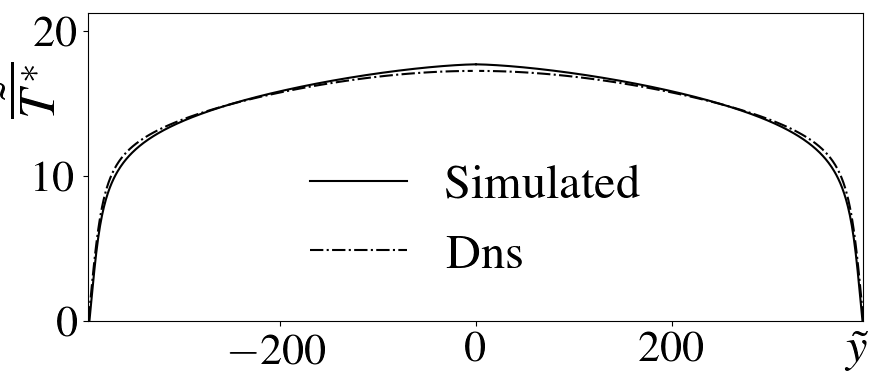
\includegraphics[angle=0, scale=0.24]{fotos_formatacao_final/Temperature_395_071_Prt0905_A26}
		\caption{$Re_\tau = 395$, $L2_t = 0.23$}
	\end{subfigure}
	\begin{subfigure}[t]{0.5\textwidth}
		\centering
		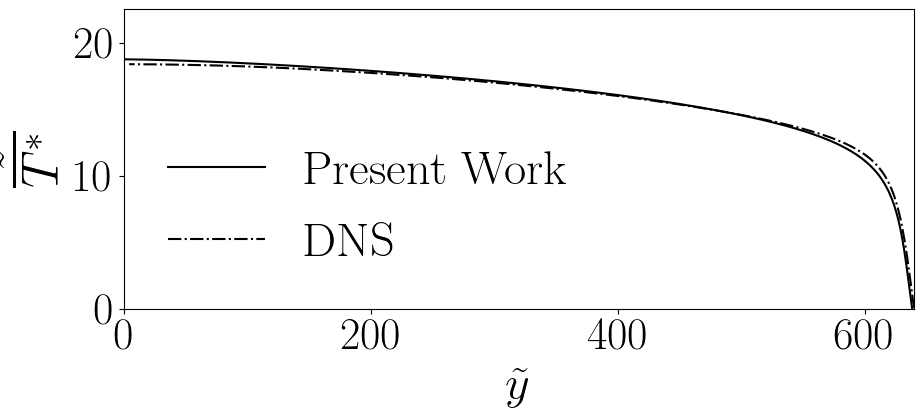
\includegraphics[angle=0, scale=0.24]{fotos_formatacao_final/Temperature_640_071_Prt0905_A26}
		\caption{for $Re_\tau = 640$, $L2_t = 0.19$}
	\end{subfigure}
	\begin{subfigure}[t]{0.45\textwidth}
		\centering
		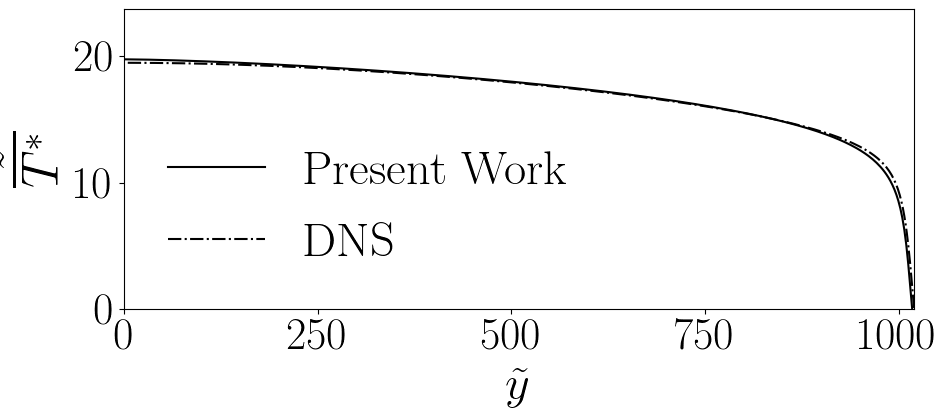
\includegraphics[angle=0, scale=0.24]{fotos_formatacao_final/Temperature_1000_071_Prt0905_A26}
		\caption{for $Re_\tau = 1020$, $L2_t = 0.14$}
	\end{subfigure}	
	\caption{Results of temperature simulations for $Pr_t = 0.9 $, $A = 26$ and $Pr =0.71$ }
	\label{primeiros}
\end{figure*}

Although the results were much better as compared with figure \ref{figuraresultados1}, the model had to be further improved. The turbulent Prandtl number varies with the Reynolds number as observed on (fig.\ref{figure5}), so a model that contemplate this fact had to be proposed. 
In order to obtain a curve for $Pr_t$ as a function of $Re_\tau$, the same optimizing algorithm had to be used to determine an ideal turbulent Prandtl number for each turbulent Reynolds number available in the DNS data base \cite{DNS1020} and \cite{DNS150}.
The best turbulent Prandtl numbers obtained are summarized in table \ref{tabela1}:

\begin{table}[!h]
	\centering
	\caption{Ideal turbulent Prandtl Numbers adjusted for each Reynolds number, with the Cebeci constant $A = 26$}
	\begin{tabular}{ll}
		  \hline
		  $Re_\tau$ & $Pr_t$\\
		  \hline
		  150  &   0.94531\\
		  395  &   0.89531\\
		  640  &   0.89531\\
		  1020 &   0.90000\\ 
		  \hline
	\end{tabular}
	\label{tabela1}
\end{table}



By performing a polynomial curve fit, a model adjusted for the turbulent Prandtl number as a function of the Reynolds number was developed:
\begin{equation}
\begin{split}
Pr_t = -4.5604 * 10^{-10} Re_\tau^3 + 9.5690 * 10^{-7} Re_\tau^2 - 6.1715 *10 ^{-4} Re_\tau + 1.0178 .
\end{split}
\end{equation}
The result of the simulations were much accurate, even more than the simulations with the turbulent Prandtl numbers set as the mean values of the ones from the DNS data (fig.\ref{figure5}). These results can be seen in figure \ref{figura_9}:



\begin{figure*}[!h]
	\centering
	\begin{subfigure}[t]{0.5\textwidth}
		\centering
		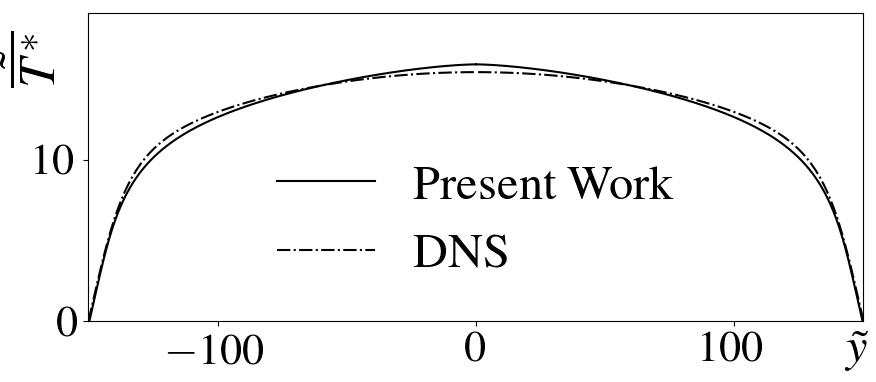
\includegraphics[angle=0, scale=0.24]{fotos_formatacao_final/Temperature_150_071_Prt(Ret)_A26}
		\caption{$Re_\tau = 150$, $L2_t = 0.26$}
	\end{subfigure}
	\begin{subfigure}[t]{0.45\textwidth}
		\centering
		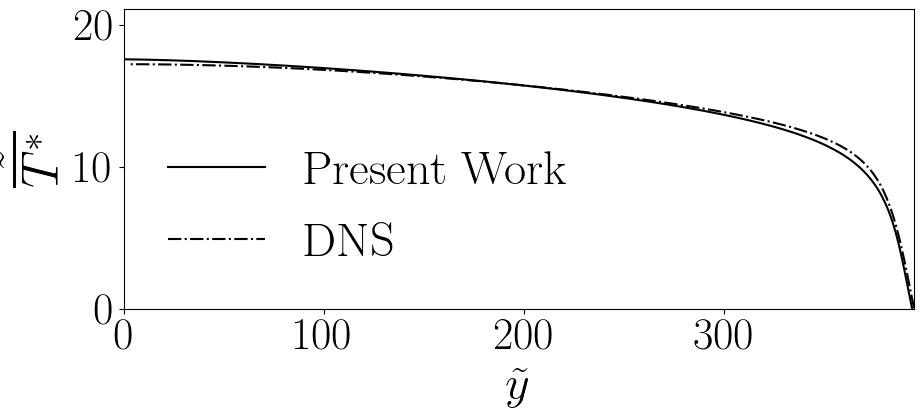
\includegraphics[angle=0, scale=0.24]{fotos_formatacao_final/Temperature_395_071_Prt(Ret)_A26}
		\caption{$Re_\tau = 395$, $L2_t = 0.22$}
	\end{subfigure}
	\begin{subfigure}[t]{0.5\textwidth}
		\centering
		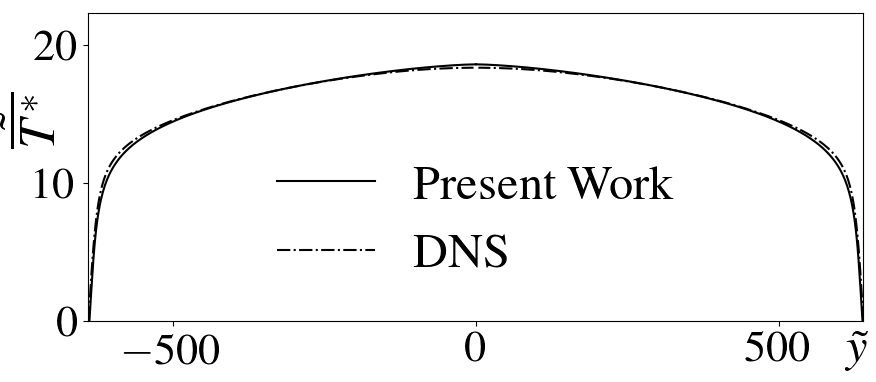
\includegraphics[angle=0, scale=0.24]{fotos_formatacao_final/Temperature_640_071_Prt(Ret)_A26}
		\caption{$Re_\tau = 640$, $L2_t = 0.17$}
	\end{subfigure}
	\begin{subfigure}[t]{0.45\textwidth}
		\centering
		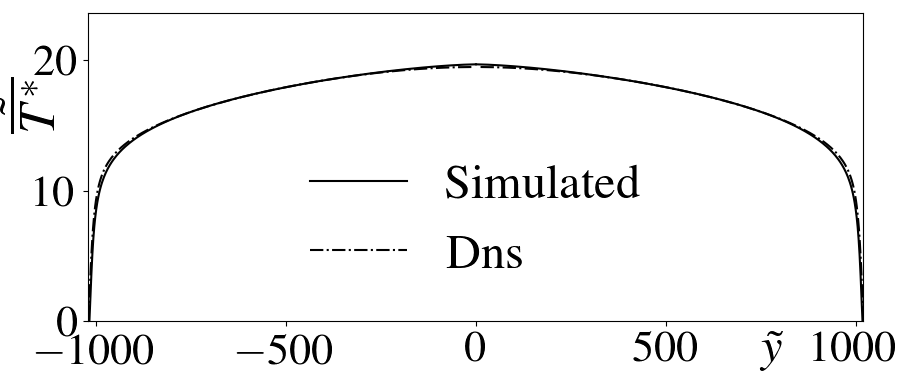
\includegraphics[angle=0, scale=0.24]{fotos_formatacao_final/Temperature_1000_071_Prt(Ret)_A26}
		\caption{$Re_\tau = 1020$, $L2_t = 0.14$}
	\end{subfigure}	
	\caption{Results of temperature simulations for $Pr_\tau(Re_\tau)$, $A = 26$ and $Pr =0.71$. }
	\label{figura_9}
\end{figure*}



\newpage

Other manners of reducing the inaccuracy were searched. The velocity profile was a possibility as it plays an important role in the error of the method. Simulations were carried developing just this physical property, and there was error associated too (fig.\ref{figura_10}).

\begin{figure*}[!h]
	\centering
	\begin{subfigure}[t]{0.5\textwidth}
		\centering
		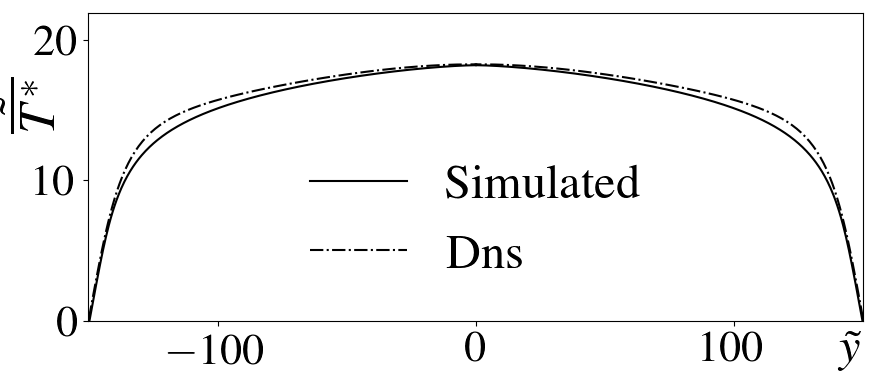
\includegraphics[angle=0, scale=0.24]{fotos_formatacao_final/Temperature_150_Avelocity}
		\caption{$Re_\tau = 150$, $L2_d = 0.47$}
	\end{subfigure}
	\begin{subfigure}[t]{0.45\textwidth}
		\centering
		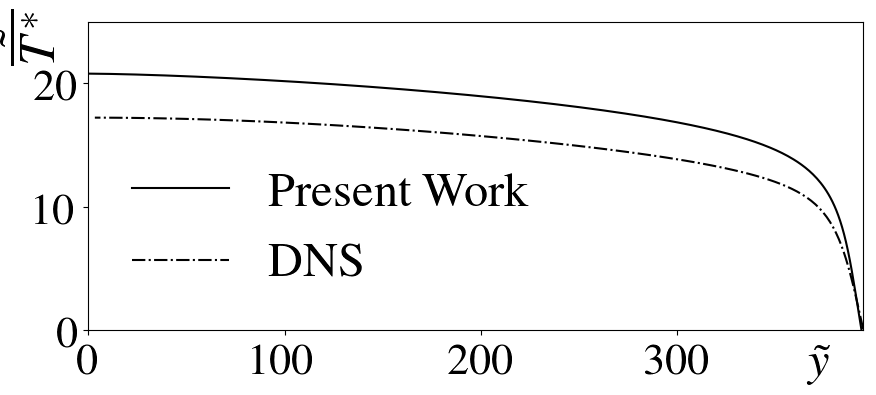
\includegraphics[angle=0, scale=0.24]{fotos_formatacao_final/Temperature_395_Avelocity}
		\caption{$Re_\tau = 395$, $L2_d = 0.17$}
	\end{subfigure}
	\begin{subfigure}[t]{0.5\textwidth}
		\centering
		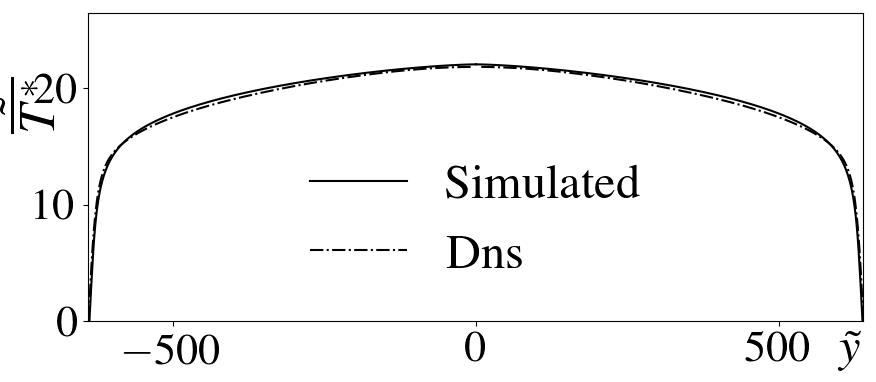
\includegraphics[angle=0, scale=0.24]{fotos_formatacao_final/Temperature_640_Avelocity}
		\caption{$Re_\tau = 640$, $L2_d = 0.23$}
	\end{subfigure}
	\begin{subfigure}[t]{0.45\textwidth}
		\centering
		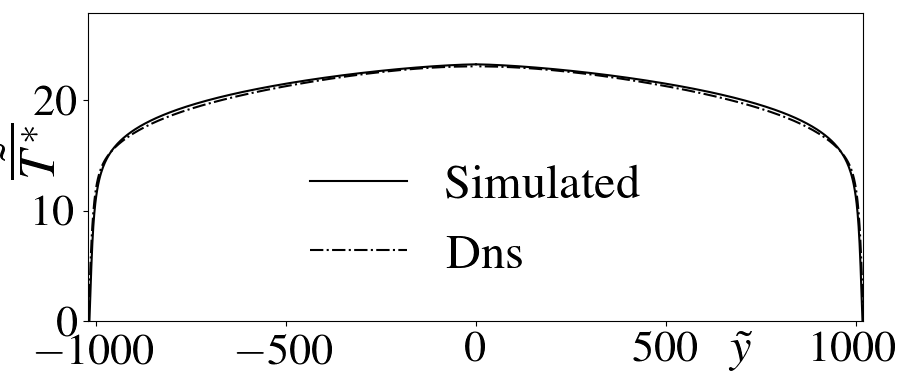
\includegraphics[angle=0, scale=0.24]{fotos_formatacao_final/Temperature_1000_Avelocity}
		\caption{$Re_\tau = 1020$, $L2_d = 0.23$}
	\end{subfigure}	
	\caption{Results of velocity simulations for $A = 26$}
	\label{figura_10}
\end{figure*}


A adjusted model was proposed in the present work for the Cebeci's constant $A$ aiming to reduce it's error, and by extension, making the method more accurate. The same algorithm used to find the ideal turbulent Prandtl numbers was used to find an ideal Cebecis's constant for each turbulent Reynolds number. It was used the velocity from DNS available to calculate de L2 norm. The Cebeci constant "A" was defined as an editable variable for the program, and the L2 norm was set as a parameter of interest. The results for ideal Cebeci's constants can be seen ahead.

\newpage

\begin{table}[!h]
	\centering
	\caption{Ideal Cebeci's constant adjusted for each Reynolds number}
	\begin{tabular}{ll}
		\hline
		$Re_\tau$ & $A$\\
		\hline
		150  &   28.616180\\
		395  &   25.673782\\
		640  &   25.001266\\
		1020 &   25.002136\\ 
		\hline
	\end{tabular}
	\label{tablea}
\end{table}

 From the resulting points of the optimization algorithm, a model was prepared and adjusted for a kind of Cebeci function:
\begin{equation}
A \left( Re_\tau\right)= \frac{Re_\tau ^{0.0451 * \ln(Re_\tau)} *e ^ {5.2753} }{Re_\tau ^{0.6094}}.
\end{equation}

Then, it result in an adjusted method for the proposed Cebeci's function, optimized using minimal error relative to the velocity, as can be seen in the simulations, there was a improvement on the velocity calculation:


\begin{figure*}[!h]
	\centering
	\begin{subfigure}[t]{0.5\textwidth}
		\centering
		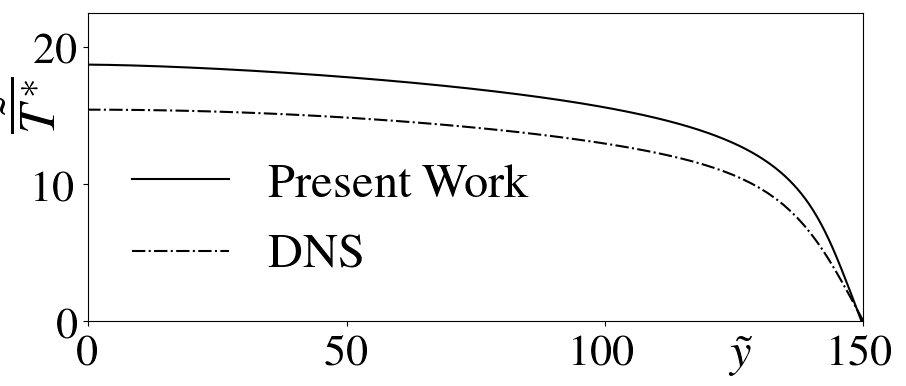
\includegraphics[angle=0, scale=0.24]{fotos_formatacao_final/Temperature_150_Amodeled}
		\caption{$Re_\tau = 150$, $L2_d = 0.28$}
	\end{subfigure}
	\begin{subfigure}[t]{0.45\textwidth}
		\centering
		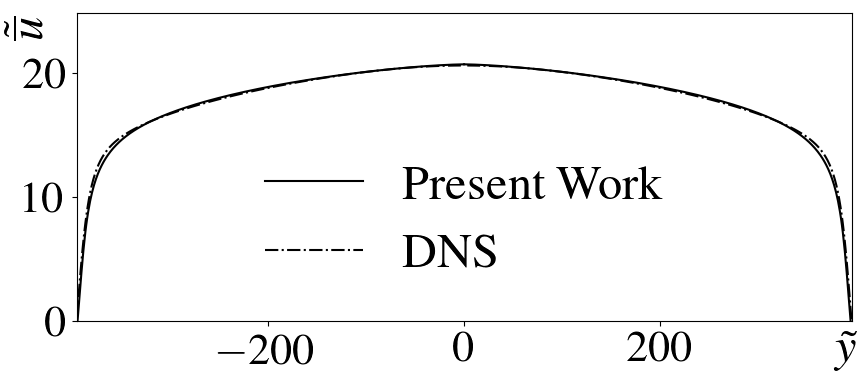
\includegraphics[angle=0, scale=0.24]{fotos_formatacao_final/Temperature_395_Amodeled}
		\caption{$Re_\tau = 395$, $L2_d = 0.16$}
	\end{subfigure}
	\begin{subfigure}[t]{0.5\textwidth}
		\centering
		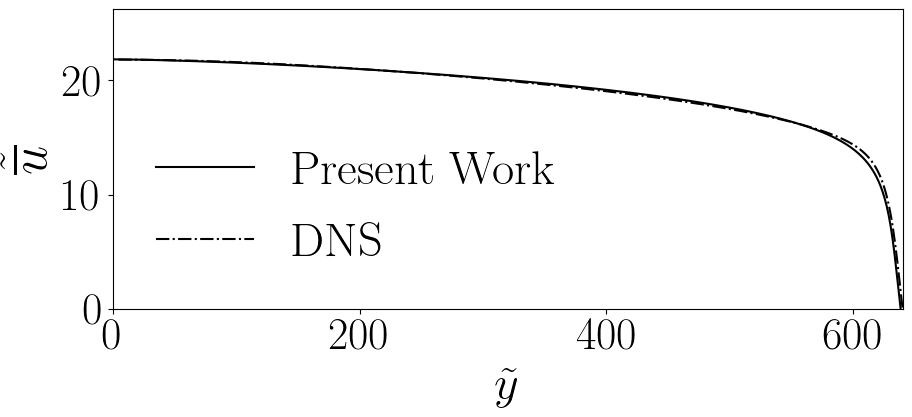
\includegraphics[angle=0, scale=0.24]{fotos_formatacao_final/Temperature_640_Amodeled}
		\caption{$Re_\tau = 640$, $L2_d = 0.14$}
	\end{subfigure}
	\begin{subfigure}[t]{0.45\textwidth}
		\centering
		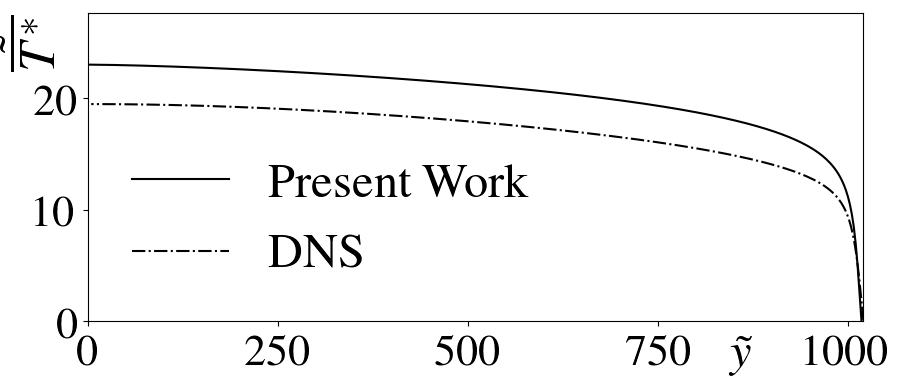
\includegraphics[angle=0, scale=0.24]{fotos_formatacao_final/Temperature_1000_Amodeled}
		\caption{$Re_\tau = 1020$, $L2_d = 0.13$}
	\end{subfigure}	
	\caption{Results in velocity distribution for A modeled.}
\end{figure*}

With the Cebeci's function adjusted, a new group of optimizations were made, with the same differential evolution methodology, taking into consideration this new formulation for the Cebeci's constant. Such study resulted in a new set of optimal turbulent Prandtl number for each DNS sample Reynolds number, as follows:


\begin{table}[!h]
	\centering
	\caption{Ideal turbulent Prandtl Numbers adjusted for each turbulent Reynolds number, with the Cebeci's function modeled. }
	\begin{tabular}{ll}
		\hline
		$Re_\tau$ & $Pr_t$\\
		\hline
		150  &   0.88594\\
		395  &   0.90156\\
		640  &   0.91094\\
		1020 &   0.91406\\ 
		\hline
	\end{tabular}
\end{table}

A new model could be proposed for the Turbulent Prandtl number.
	\vspace{-2mm}
\begin{equation}
\begin{split}
Pr_t = 4.5290 * 10^{-12} Re_\tau^3 - 5.7395 * 10^{-8} Re_\tau^2 + 9.397 * 10^{-5} Re_\tau + 0.8731.
\end{split}
\end{equation}


With such parametrization, a new set of simulations were made, with the following results:

\begin{figure*}[!h]
	\centering
	\begin{subfigure}[t]{0.5\textwidth}
		\centering
		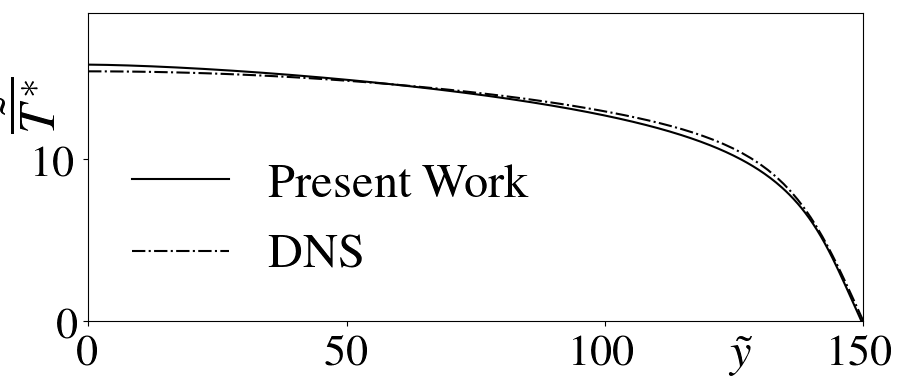
\includegraphics[angle=0, scale=0.24]{fotos_formatacao_final/Temperature_150_071_Prt(Ret)_Avelocity}
		\caption{$Re_\tau = 150$, $L2_t = 0.212$}
	\end{subfigure}
	\begin{subfigure}[t]{0.45\textwidth}
		\centering
		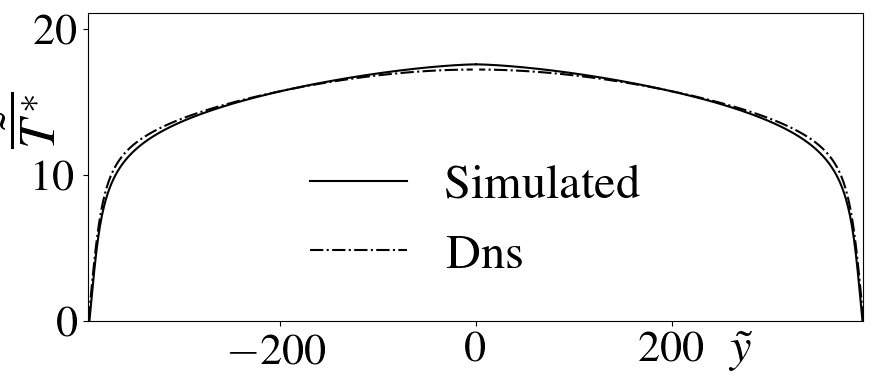
\includegraphics[angle=0, scale=0.24]{fotos_formatacao_final/Temperature_395_071_Prt(Ret)_Avelocity}
		\caption{$Re_\tau = 395$, $L2_t = 0.233$}
	\end{subfigure}
	\begin{subfigure}[t]{0.5\textwidth}
		\centering
		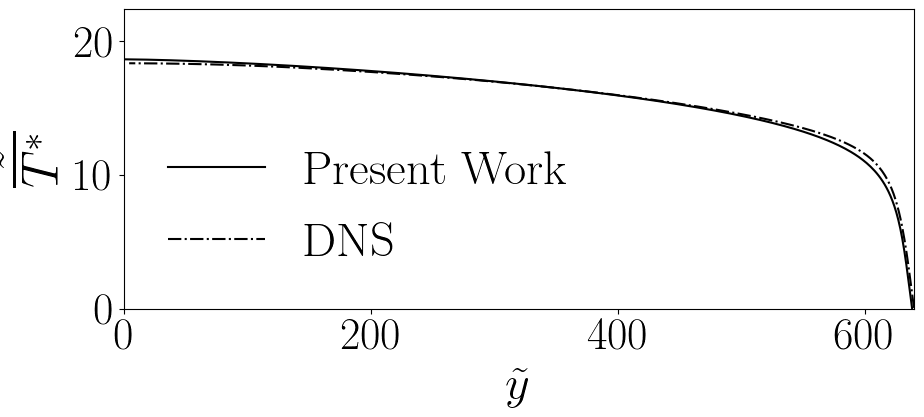
\includegraphics[angle=0, scale=0.24]{fotos_formatacao_final/Temperature_640_071_Prt(Ret)_Avelocity}
		\caption{$Re_\tau = 640$, $L2_t = 0.205$}
	\end{subfigure}
	\begin{subfigure}[t]{0.45\textwidth}
		\centering
		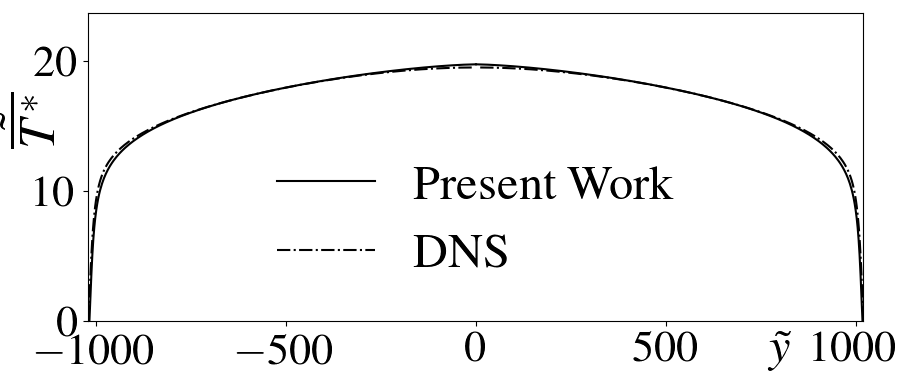
\includegraphics[angle=0, scale=0.24]{fotos_formatacao_final/Temperature_1000_071_Prt(Ret)_Avelocity}
		\caption{$Re_\tau = 1020$, $L2_t = 0.175$}
	\end{subfigure}	
	\caption{Results of temperature simulations for $Pr_\tau(Re\tau)$, $A(Re_\tau)$ and $Pr =0.71$ }
\end{figure*}

The Cebeci's values that resulted in a minor error for the velocity don't had the same effect on the temperature results. The Cebeci was modeled for the minimum velocity error, not being the best for the thermal solution. Algebraically, the Cebeci's function appears two times as seen in equations \ref{equationultima} and \ref{finalequationvelocity}. Then, it is possible to propose two Cebeci's function models. One for the dynamical simulation $ A_d $, and one for the temperature simulations $ A_t $.     


Another method of adjustment on differential evolution is the multi objective adjustment. Such approach was used to consider more then one variable simultaneously for optimization. This method was used to adjust the thermal Cebeci's function and the Turbulent Prandtl number for the minor error (L2 norm) in the resulting temperature field for each DNS sample. The Cebeci function for velocity was considered in the previously development. New ideal values were found for the turbulent Prandtl number and the thermal Cebeci`s constant:

\begin{table}[!h]
	\centering
	\caption{Ideal turbulent Prandtl Numbers and thermal Cebeci`s function ($A_t$) adjusted for each turbulent Reynolds number, with the multi objective approach. The Cebeci for velocity ($A_d$) continued the same from table \ref{tablea}. }
	\begin{tabular}{llll}
		\hline
		$Re_\tau$ & $Pr_t$ & $A_t$ & $A_d$\\
		\hline
		150  &   0.72530 & 37.25510 & 28.616180\\
		395  &   0.76821 & 34.24176 & 25.673782\\
		640  &   0.81896 & 31.27627 & 25.001266\\
		1020 &   0.86179 & 28.73726 & 25.002136\\ 
		\hline
	\end{tabular}
\end{table}
With such numerical DATA, new models were both proposed for the Turbulent Prandtl number and the thermal Cebeci`s function:

\begin{equation}
A_t = \frac{Re_\tau ^{0.0395 \ln(Re_\tau)^2 - 0.7588 \ln(Re_\tau) +  4.6637  } }{e ^{5.6703}},
\end{equation}

\begin{equation}
\begin{split}
Pr_t = -2.4892 * 10^{-10} Re_\tau^3 +  3.6036 * 10^{-7} Re_\tau^2 + 3.7921 *10 ^{-5} Re_\tau + 0.7123 .
\end{split}
\end{equation}
More simulations were developed using such new proposed models.

\begin{figure*}[!h]
	\centering
	\begin{subfigure}[t]{0.5\textwidth}
		\centering
		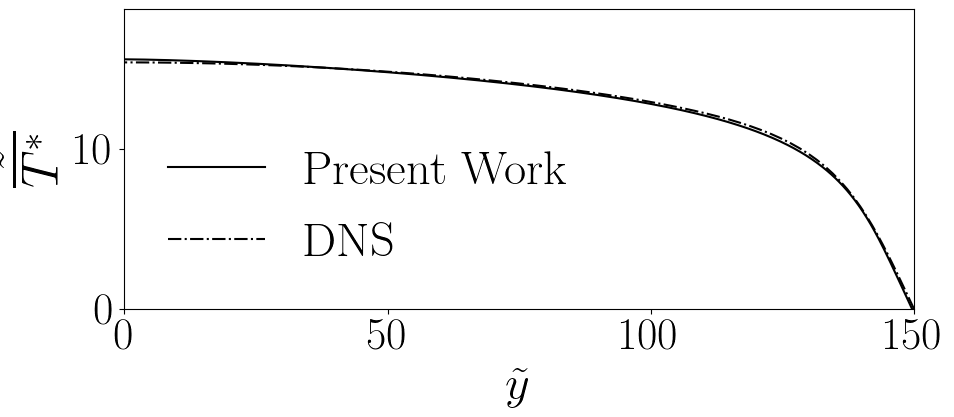
\includegraphics[angle=0, scale=0.24]{fotos_formatacao_final/Temperature_150_071_Genetic2temperature}
		\caption{$Re_\tau = 150$, $L2_t = 0.091$}
	\end{subfigure}
	\begin{subfigure}[t]{0.45\textwidth}
		\centering
		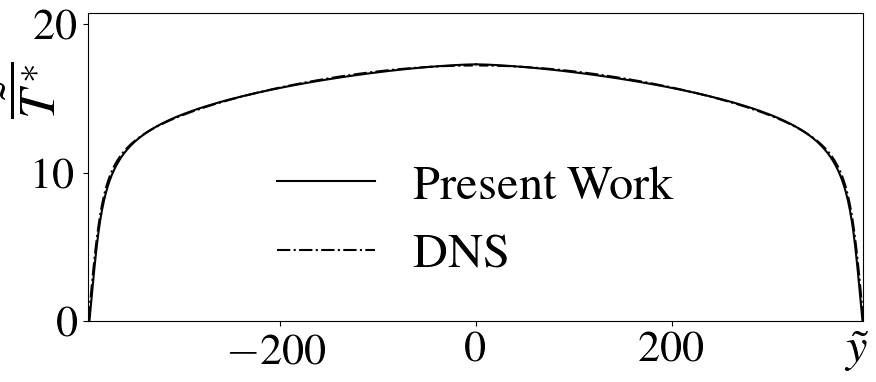
\includegraphics[angle=0, scale=0.24]{fotos_formatacao_final/Temperature_395_071_Genetic2temperature}
		\caption{$Re_\tau = 395$, $L2_t = 0.049$}
	\end{subfigure}
	\begin{subfigure}[t]{0.5\textwidth}
		\centering
		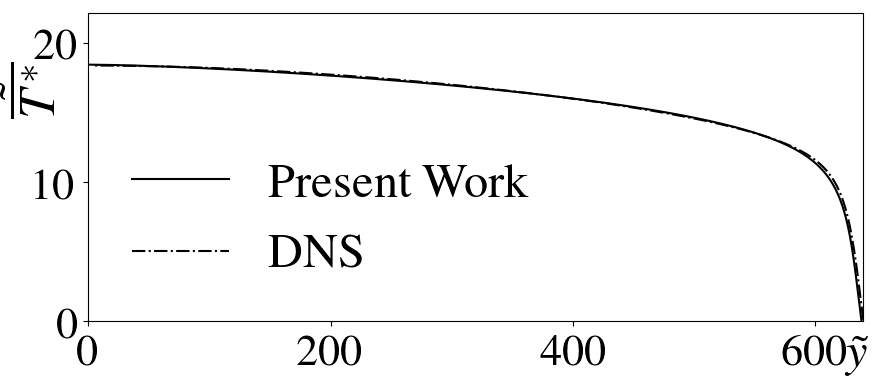
\includegraphics[angle=0, scale=0.24]{fotos_formatacao_final/Temperature_640_071_Genetic2temperature}
		\caption{$Re_\tau = 640$, $L2_t = 0.061$}
	\end{subfigure}
	\begin{subfigure}[t]{0.45\textwidth}
		\centering
		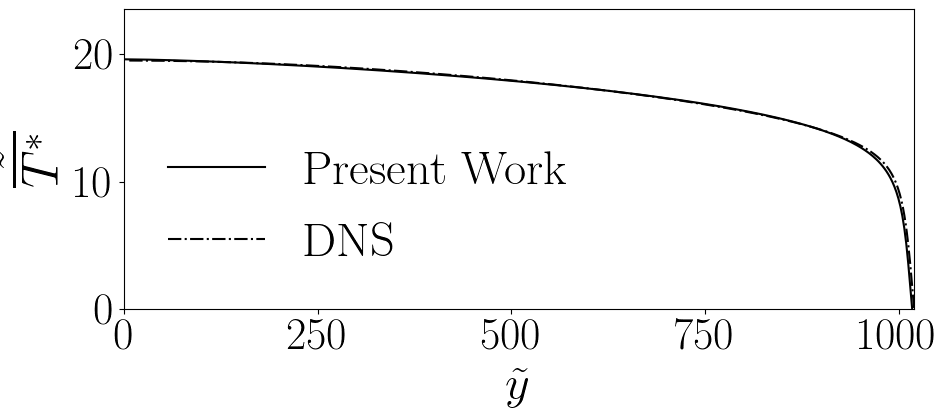
\includegraphics[angle=0, scale=0.24]{fotos_formatacao_final/Temperature_1000_071_Genetic2temperature}
		\caption{$Re_\tau = 1020$, $L2_t = 0.076$}
	\end{subfigure}	
	\caption{Results of temperature simulations for $Pr_\tau(Re_\tau)$, $A_d(Re_\tau)$, $A_t(Re_\tau) $ and $Pr =0.71$, with multi-objective adjustment.}
	\vspace{-5mm}
\end{figure*}





 
\section{Results}

With such methods, it was studied the advantages and disadvantages of each one. A comparison between errors can be seen ahead, in figure \ref{figure15}:\\

\begin{figure}[!h]
	\centering
	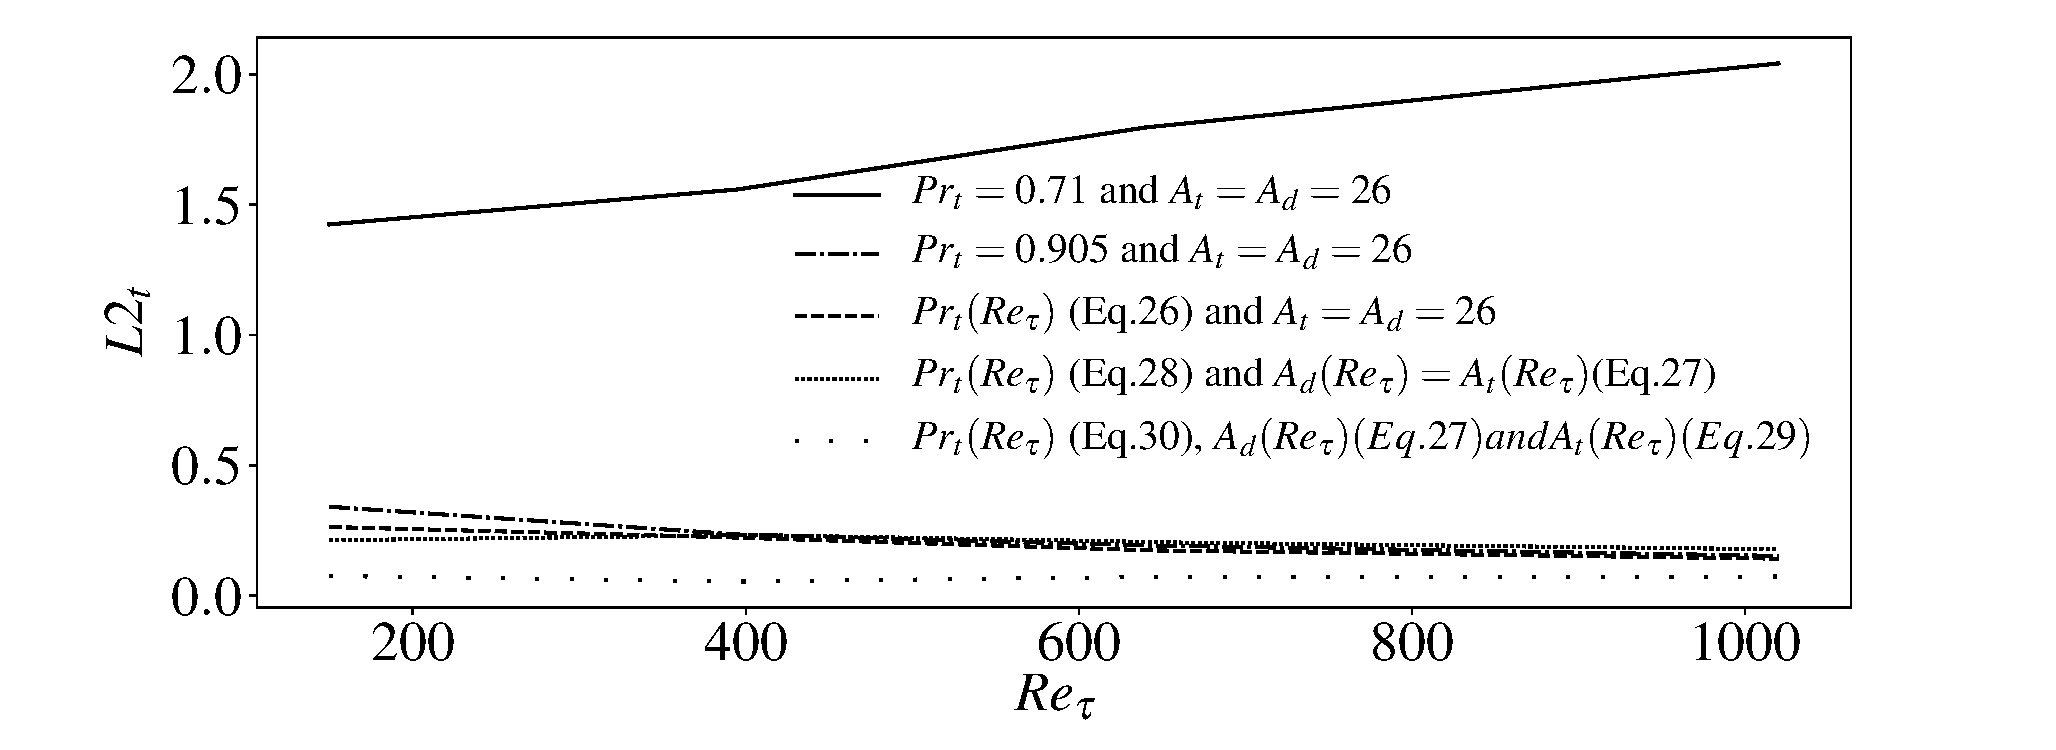
\includegraphics[angle=0, trim = {20mm 0mm 0mm 10mm}, scale=0.5]{fotos_formatacao_final/gerais}
	\caption{Comparison between all proposed models for $Pr_t$, $A_d$ and $A_v$, in respect to the temperature results in comparison with DNS.}
	\label{figure15}
\end{figure}

All the models developed on the present paper shown better results then the classical parametrization of $Pr_t = 0.71$ and $A = 26$ on the turbulent Poiseuille flow. The correction in the Cebeci's constant, although represented a smaller error in the velocity, didn't resulted in smaller errors in the temperature profile for all the domain. The model that presents the best results was the developed with the multi-objective differential evolution algorithm in with it was considered two Cebeci's functions for each domain (thermal and dynamical).\\

The dynamical Cebeci's constant optimization caused gains in the velocity field in terms of velocity error, as seen in figure \ref{figure16}.

\begin{figure}[!h]
	\centering
	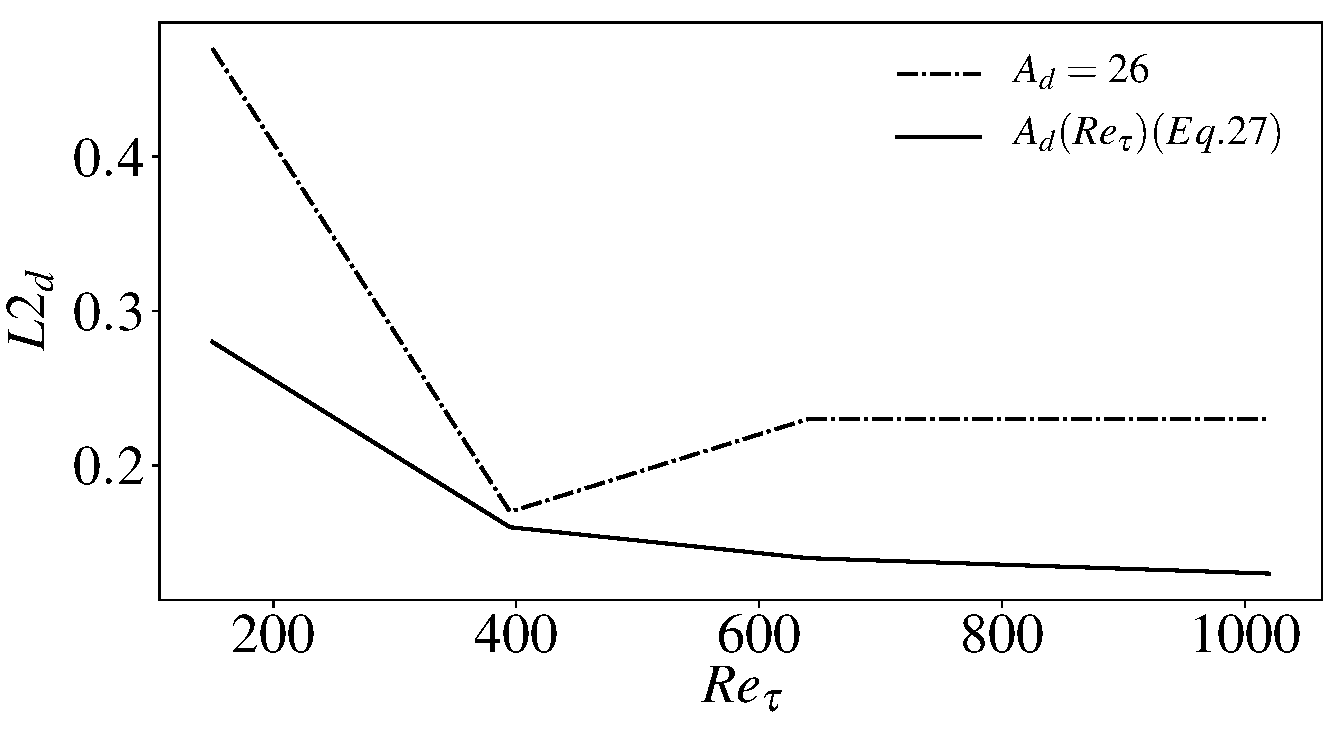
\includegraphics[angle=0, trim = {0mm 0mm 0mm 10mm}, scale=0.5]{fotos_formatacao_final/gerais_velo}
	\caption{Comparison between the proposed models for $A_d$, in respect to the velocity results in comparison with DNS.}
	\label{figure16}
\end{figure}

\section{Conclusion}

In the present paper it was successfully developed a semi-analytical methodology to calculate the temperature profile inside a channel with the Prandtl mixing length model, a classic closure model in the study of turbulence. The validations with DNS were satisfactory. Its is important to notice that such values of turbulent Prandtl number and Cebeci's function were applied for this particular case, as the parametrizations were particular computational adjustments and there are simplifications of the physical abstractions that each model represents. But they suited well for this case, resulting in accuracy and efficiency. The semi analytical method was successful in model the problem, as good results were obtained when used the turbulent Prandtl numbers from the DNS. As for the models proposed, it is an idea to test then in other problems, with other geometries and using other kinds of turbulence closure models, as a way of testing their usability for other problems.      

\section{Acknowledgments}

It's opportune to thanks all the institutions involved with the viabilization of the present research project. The laboratory of fluids mechanic (MFLab) of the Mechanical Engineering College (FEMEC) of the Federal University of Uberlandia (UFU). PETROBRAS, CNPq, CAPES and FAPEMIG that contributed financially to this project.  

\begin{thebibliography}{99} % Bibliography - this is intentionally simple in this template
	
	
	\bibitem{hasan}
	{O. , Basim and Hasan}
	\newblock  {"Turbulent Prandtl Number and its Use in Prediction of Heat Transfer Coefficient for liquids."}
	\newblock {Nahrain University, College of engineering Journal (NUCEJ) Vol.10, No.1}
	\newblock {2007}.
	
	
	\bibitem{Poiseuille}
	{J. , L. ,  M. , Poiseuille},
	\newblock{"Recherches experimentales sur Ie mouvement des liquides dans les tubes de tres-petits diametres"},
	\newblock{Memoires presentes par divers savants a l'Academie Royale des Sciences de l'Institut de France},
	\newblock{IX: 433-544},
	\newblock{1846}.
	
	
	\bibitem{Prandtl}
	\newblock{L. , Prandtl},
	\newblock{Uber die ausgebildete Turbulenz},
	\newblock{ZAMM},
	\newblock{1925}.
	
	
	\bibitem{Cebeci}
	{T. , Cebeci and P. , Bradshaw},
	\newblock{"Physical and computational aspects of convective heat transfer"},
	\newblock{Springer},
	\newblock{New York},
	\newblock{1984}.
	
	
	\bibitem{John}
	\newblock{John , C.  , Sommerer and Edward , Ott and Tamas , Tel},
	\newblock{"Modeling Two-Dimensional Fluid Flows with Chaos Theory"},
	\newblock{Johns Hopkins APL Technical Digest, volume 18, number 2},
	\newblock{193-202},
	\newblock{1997}.
	
	
	\bibitem{aristeu}
	\newblock{A. S. {Neto}},
	\newblock{"Turbul\^encia nos fluidos, textbook of the post graduate mechanical engineering course of federal university of Uberl\^andia"},
	\newblock{Uberl\^andia, Brazil},
	\newblock{2018}.
	
	
	\bibitem{Cengel}
	\newblock{Y. , A., Cengel and J. , M. , Cimbala},
	\newblock{Fluid mechanics Fundamentals and Applications},
	\newblock{First edition},
	\newblock{McGraw-Hill series in mechanical engineering},
	\newblock{2006}.
	
	\bibitem{Abe}
	H. , Kawamura and H. , Abe and Yuichi , Matsuo,
	\newblock{DNS of turbulent heat transfer in channel flow with respect to Reynolds and Prandtl number effects},
	\newblock{Elsevier},
	\newblock{Tokio, Japan},
	\newblock{1999}.
	
	
	\bibitem{Kawamura}
	Kawamura, H. , Abe, H. and shingai, k. ,
	\newblock {"DNS of turbulence and heat transport in a channel flow with different Reynolds and Prandtl numbers and boundary conditions."},
	\newblock { Turbulence, Heat and Mass Transfer 3, (Proc. of the 3rd International Symposium on Turbulence, Heat and Mass Transfer)},
	\newblock {2000}.
	
	
	\bibitem{Incropera}
	Incropera, Freank, P., Dewitt, David, P.,  
	\newblock {\em fundamentals of Heat and Mass Transfer}, 3rd edition,
	\newblock p. 310-316, 2007, LTC,
	\newblock (INCROPERA and DEWITT).
	
	\bibitem{DNS1020}
	H Kawamura,
    \newblock{Direct Numerical Simulation Data Base for Turbulent Channel Flow with Heat Transfer.},
	\newblock{<http://www.rs.tus.ac.jp/~t2lab/db/index.html>, Laboratory of Thermo-fluid dynamics, Department of Mechanical Engineering, Faculty of Science and Technology, Tokyo University of Science, Noda-shi, Chiba-ken, Japan},
	\newblock{2007}.	
	
	
	\bibitem{DNS150}
	N Kasagi and K Horiuti and Y Miyake and T Miyauchi and Y Nagano ,
	\newblock{Establishment of the Direct Numerical Simulation Data Bases of Turbulent Transport Phenomena},
	\newblock{<http://thtlab.jp/DNS/dns\_database.html>,  Co-operative Research No. 02302043, Bunkyo-ku, Tokyo 113  },
	\newblock{1992}.
	
	
	\bibitem{Luigi}
	L A Antonialli and A N Silveira ,
	\newblock{Theoretical study of fully develop turbulent flow in a flat channel, using prandtl's
mixing length model},
	\newblock{2015}.
	
	
	
\end{thebibliography}





\end{document}
